
\documentclass[letterpaper,12pt,]{article}

\usepackage{titling}

\setlength{\droptitle}{5in}   % This is your set screw

\usepackage[%
    left=1in,%
    right=1in,%
    top=1in,%
    bottom=1.0in,%
    paperheight=11in,%
    paperwidth=8.5in%
]{geometry}%
\usepackage{comment}

\usepackage{listings}
\usepackage{graphicx}
\usepackage{amsmath}
\usepackage[section]{placeins}
\usepackage[font=small,skip=-2pt]{caption}
\usepackage{subcaption}
\usepackage{hyperref}
\usepackage{sectsty} %Resize section titles
\usepackage{titlesec} % Space before and after section
\sectionfont{\large}
\titlespacing*{\section}{0pt}{1ex plus 0.0ex minus .0ex}{1ex plus .0ex}



\lstdefinestyle{mystyle}{
    %backgroundcolor=\color{backcolour},   
    %commentstyle=\color{codegreen},
    %keywordstyle=\color{magenta},
    %numberstyle=\tiny\color{codegray},
    %stringstyle=\color{codepurple},
    basicstyle=\footnotesize,
    breakatwhitespace=false,         
    breaklines=true,                 
    captionpos=b,                    
    keepspaces=true,                 
    numbers=left,                    
    numberstyle=\footnotesize,               
    stepnumber=1,
    numbersep=5pt,
    showspaces=false,                
    showstringspaces=false,
    showtabs=false,                  
    tabsize=2,
    frame=single
}
\lstset{frame=single}

%\pagestyle{empty} % Remove page numbering
\linespread{2.0} % Line Spacing

\begin{document}
\begin{titlepage}

\newcommand{\HRule}{\rule{\linewidth}{0.5mm}} % Defines a new command for the horizontal lines, change thickness here

\center % Center everything on the page
 
%----------------------------------------------------------------------------------------
%	HEADING SECTIONS
%----------------------------------------------------------------------------------------


\textsc{\LARGE McGill University}\\[3.5cm]
\textsc{\Large Subsonic Aerodynamics}\\[0.5cm] 
\textsc{\large MECH 533}\\[2.5cm]

%----------------------------------------------------------------------------------------
%	TITLE SECTION
%----------------------------------------------------------------------------------------

{ \huge \bfseries Final Project}\\[1.5cm] % Title of your document

\HRule \\[0.4cm]
%----------------------------------------------------------------------------------------
%	AUTHOR SECTION
%----------------------------------------------------------------------------------------

\begin{minipage}{0.4\textwidth}
\begin{flushleft} \large
\emph{Name:}\\
Doug \textsc{Shi-Dong} % Your name
\end{flushleft}
\end{minipage}
~
\begin{minipage}{0.4\textwidth}
\begin{flushright} \large
\emph{Student ID:} \\
260466662\\
\end{flushright}
\end{minipage}\\[4cm]

\vfill{}
{\large December 3, 2015}\\[2cm]

\end{titlepage}

\newcommand{\rn}{Reynolds-number }

\section{Introduction}

The study of low \rn airfoils allows us to understand the underlying processes that create performance differences. The ideal airfoil shape will vary depending on its size, the speed at which it is travelling and the medium it is travelling in. The scaling effect is defined by the \rn $Re = Vc/\nu$, where $V$ is the flight speed, $c$ is the chord, and $\nu$ is the kinematic viscosity. It is a ratio of the inertial effects to the viscous effects.

The performance of an airfoil is quantified by the lift and drag coefficients $C_L$ and $C_D$. Its effectiveness can therefore be defined by the ratio $C_L/C_D$. At the critical \rn of 70,000 for a smooth airfoil, we can see a dramatic improvement of effectiveness. In the following sections, it will be shown that as the \rn increases, the lift to drag ratio improves. 
\section{Fundamentals of Fluid Mechanics}

As the fluid flows around the airfoil, there will be sections where the pressure is lower than than the far-field static pressure. This decreased pressure then has to increase back up to the far-field static pressure when it reaches the trailing edge also known as recovery. Therefore, there is the presence of an adverse pressure gradient along the surface. The adverse pressure gradient is the cause of flow separation, which greatly impairs the lifting properties of the airfoil.

In the lowest \rn range (below 30,000), the boundary layer is mostly laminar. Laminar flow is less resistant to flow separation due to adverse pressure gradients. Once separated, it quickly transitions into turbulent flow, which can then reattach itself as a turbulent boundary layer. This behavior creates a laminar separation bubble.

However, a \rn of 50,000 based on the separation bubble length is required for the flow to reattach. Therefore, airfoils with a chord resulting in a \rn less than 50,000 are too short for reattachment. This number supports the fact that there is a significant increase in performance at the critical \rn of 70,000.

At \rn of 100,000, the bubble can extend 20-30\% of the airfoil, changing the effective shape of the airfoil. For higher \rn, the bubble will shrink down to a few percent of the chord. However, increasing the angle of attack will create greater adverse pressure gradients. As a result, the small bubble can burst and form a longer bubble. This loss of efficiency cannot be immediately recovered by lowering the angle of attack, creating a hysteresis behavior.

When the \rn reaches 200,000, the laminar bubble can usually be avoided by letting the pressure recovery occur when the flow has become turbulent. Nonetheless, efficiency can further be improved by increasing the turbulent boundary layer's resistance to separation. For \rn above 1,000,000, laminar separation is rarely an issue. Efficiency is now gained by decreasing skin friction drag due to viscous effects in the boundary layer. An ideal airfoil would therefore have just enough separation resistance without the cost of adding too much skin friction drag.

It is important to note that the separation behavior depends on the local boundary layer \rn. Therefore, it is still possible for laminar separation to occur for very high \rn e.g. thin airfoils with small nose at high angle of attack.

Since turbulent boundary layers are more resistant to separation than laminar ones, it is sometimes desirable to artificially accelerate transition. This can be done mechanically through surface roughness or even vibrations. 

%It is hard to properly design turbulators since they only need to create enough turbulence to keep the boundary layer from separating.

\section{Experimental Testing of Airfoils}

Multiple issues arise when it comes to experimental testing of airfoils. Correlating lift and drag is difficult due to the different in orders of magnitude of around 100. Furthermore, stall and separation are usually the regions of interest, but they are also the regions where small changes lead to big differences.

Windtunnel results often suffer from the wall effects. The walls lead to an internal flow problem as opposed external. Also, the boundary layer from the walls may affect the flow around the airfoil. Free-flight testing allows to eliminate wall effects. However, it becomes hard to determine the performance of the airfoil only since three-dimensional effects and non-airfoil parts both affect the performance.


Therefore, experimental results often show inconsistencies from one test to another, which makes it hard for designers to rely upon them.

\section{Theoretical Design of Airfoils}

Although low \rn airfoils may operate at high Mach numbers where compressibility effects are significant and may be used in applications where three-dimensional effects are not negligible, we only consider two-dimensional incompressible flows since they very well understood.

Using complex analysis and conformal transformations, it is possible to derive exact analytical solutions of the flow field around the airfoil. Furthermore, the solution can be computed very quickly with computers. As long as the boundary layer stays attached, the solution gives a decent approximation of the airfoil performance. 

For high \rn (above 1,000,000), lift and drag can be calculated with high precision as long as there is no separation. Since transition usually occurs near the minimum pressure point, it is possible to avoid the early separation by carefully designing the airfoil in that section to reduce the adverse pressure gradient.

Design procedures can be direct or inverse. The direct procedure finds the flow field solution of a given airfoil, whereas the inverse procedure finds the airfoil shape given a pressure field. These methods are valid for attached flow with a \rn under 300,000. For lower \rn, where laminar separation and bubble occur, there are no generally accepted methods to calculated those peculiar phenomena.

\section{Special-Purpose Airfoils}

Depending on the design requirements, the airfoil shape may take very different forms. For example given an upper surface geometry and a desired lift, the pressure distribution can be defined. Inverting the pressure field allows to find the full airfoil shape, as it was the case for the BoAR 80. Another example is the Lissaman-Hibbs 8025 that required a flat upper surface for the solar cells it carried. Knowing desirable features of the pressure field and how the shape affects it allows the designers to create a nose section and undersurface that will meet the required lift and drag coefficients.

\section{Conclusion}

The study of low \rn airfoils can qualitatively explain the difference in performance as a result of transition, separation and reattachment. 

\newpage
\pagenumbering{gobble}

\section*{Question 1 Error Plot}

\begin{figure}[h!]
  \centering
  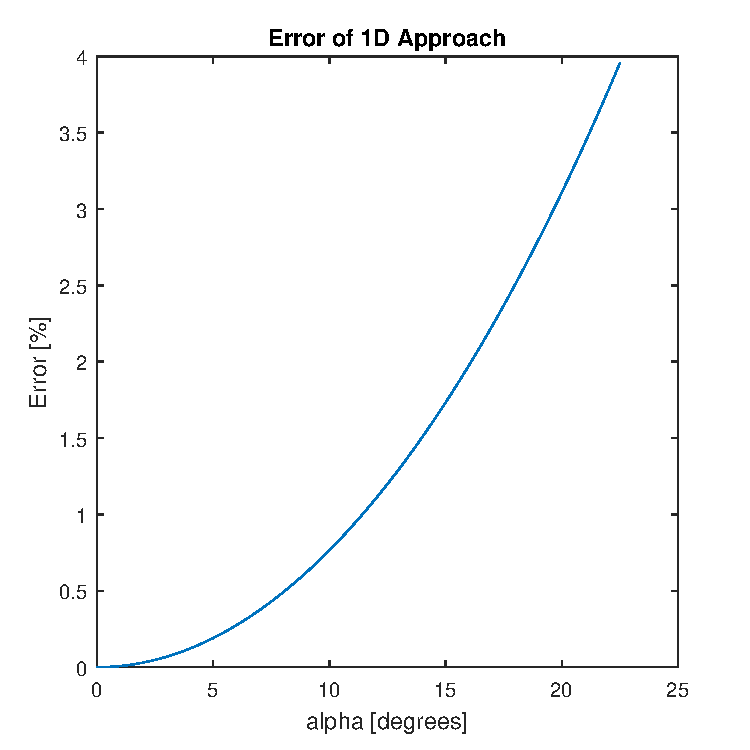
\includegraphics[width=0.9\textwidth]{plotq1}
\end{figure}

\newpage
\section*{Question 7}
\begin{figure}[h!]
  \centering
  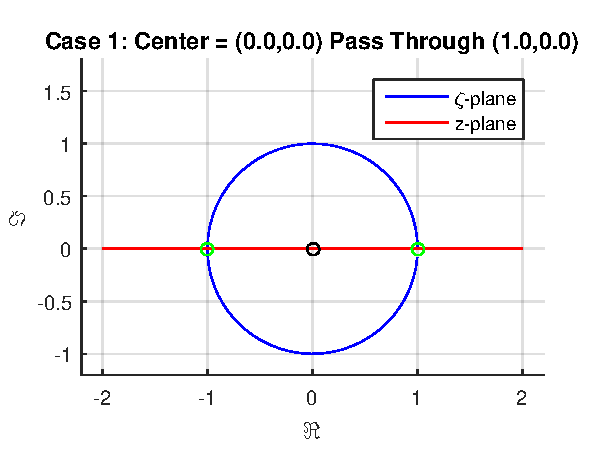
\includegraphics[width=0.40\textwidth]{case1}
  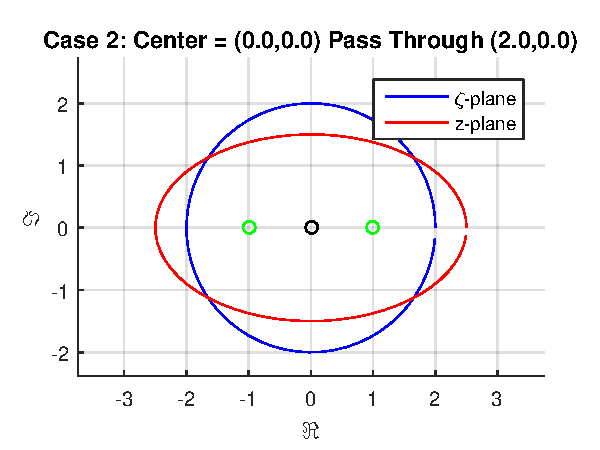
\includegraphics[width=0.40\textwidth]{case2}
  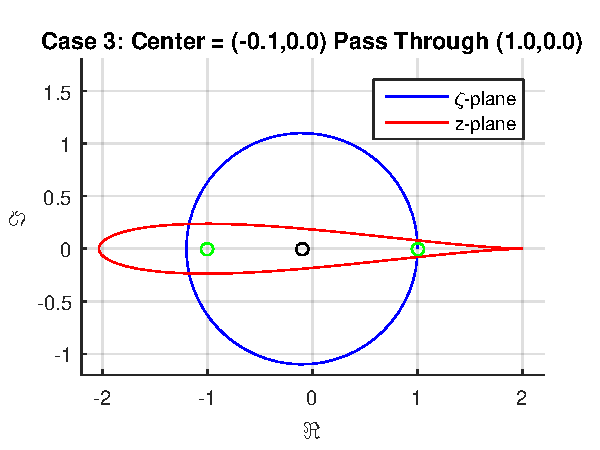
\includegraphics[width=0.40\textwidth]{case3}
  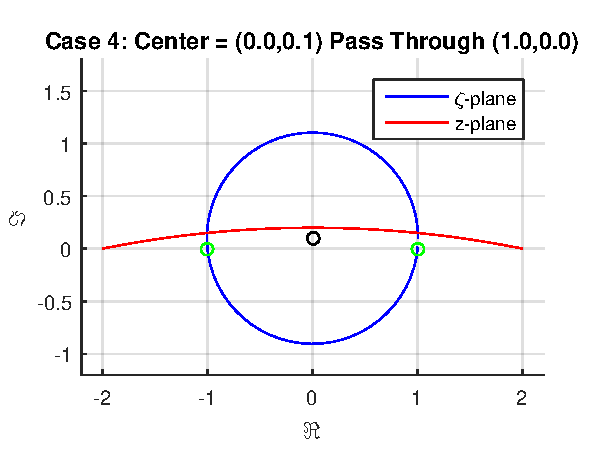
\includegraphics[width=0.40\textwidth]{case4}
  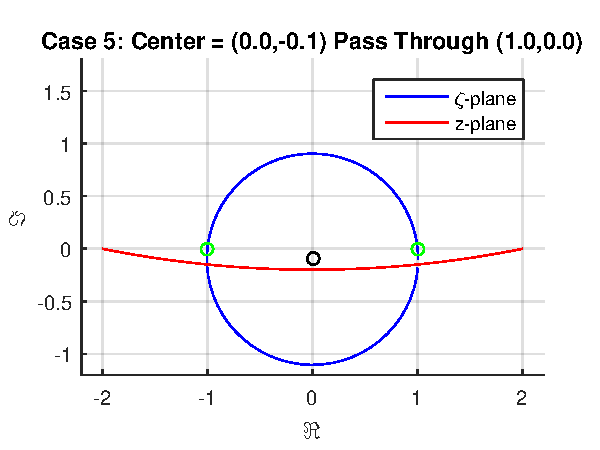
\includegraphics[width=0.40\textwidth]{case5}
  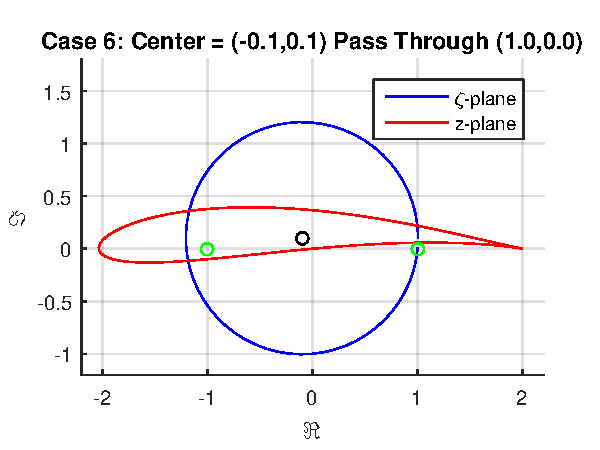
\includegraphics[width=0.40\textwidth]{case6}
  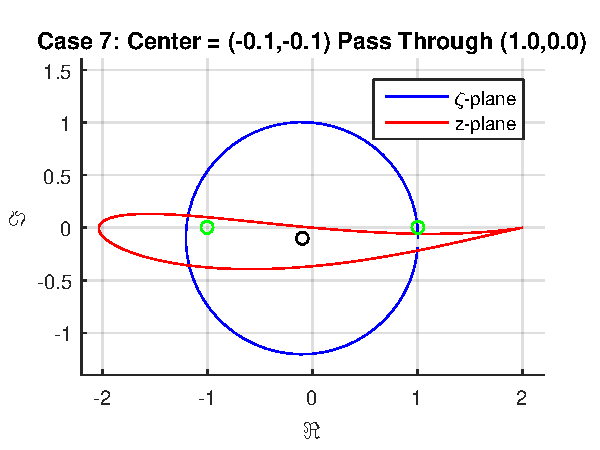
\includegraphics[width=0.40\textwidth]{case7}
\end{figure}


\end{document}

